\chapter{Report and discussion of research results}

\section{Comparison between miscalibrations of Hidden Markov Models and Condition Random Fields}

We suspect that the characteristic of a probabilistic model is a factor that affects miscalibration in structure predictions. Therefore, we choose to compare between the two most widely used classes of models in structure predictions, Hidden Markov Models (HMMs) and Conditional Random Fields (CRFs). They are fundamentally different in their objective functions: HMMs are generative models which learn the joint distribution of the observations and the labels whereas CRFs are discriminative and model directly the conditional distribution of the observations given the labels. We perform our experiements on two common structure prediction tasks: part-of-speech tagging (POS) and named-entity recognition. 

\subsection{Part-of-speech tagging}

\subsubsection{Data}

We extract articles from the Wall Street Journal (WSJ) from the CoNLL-2011 dataset for this experiment. The CoNLL has already been splitted the into training, development and testing sets so we only have to filter WSJ articles from those sets and join sentences in each set of articles into a single file. This process results in 11772 sentences for training, 1632 sentences for development and 1382 sentences for testing. The predictions we are testing is whether a word has the ``NN'' tag. 

\subsubsection{Results}

\begin{figure}[t]
\minipage{0.32\textwidth}
  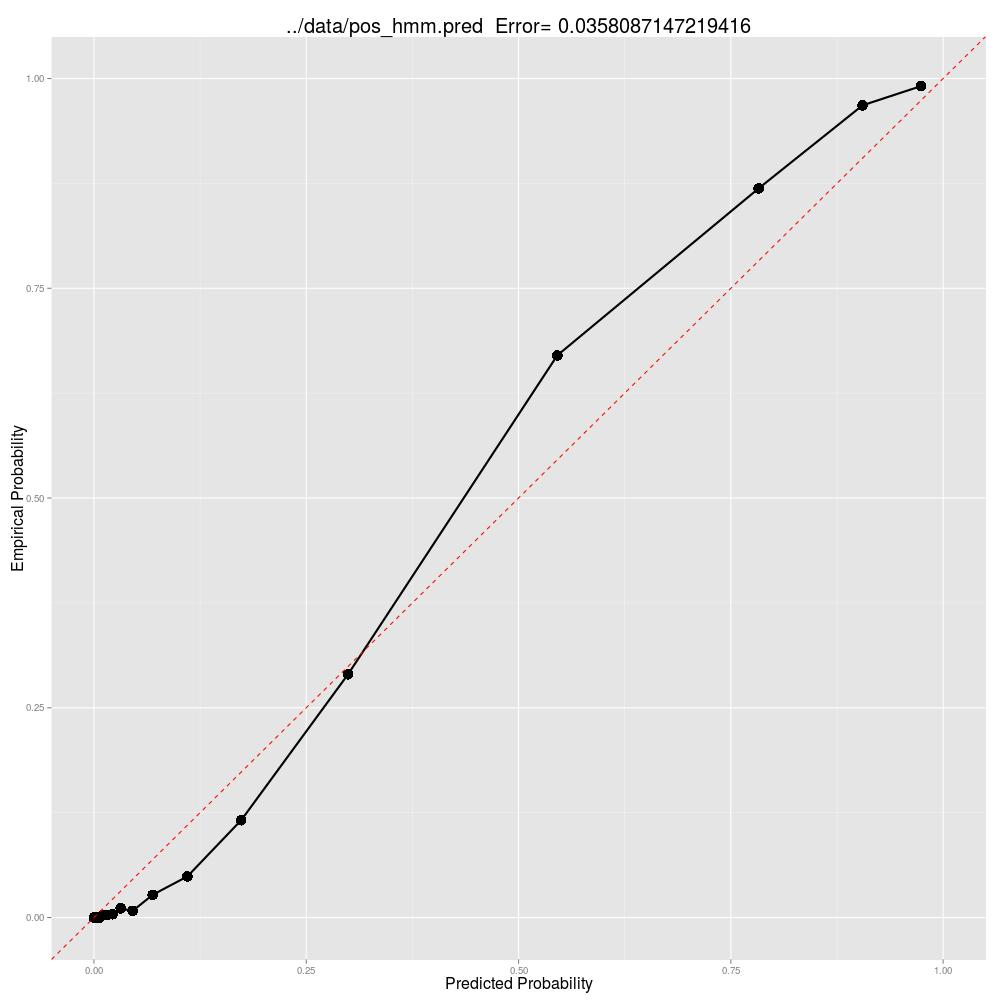
\includegraphics[width=\linewidth]{pos_hmm_pred.jpg}
  \caption{Calibration curve for HMM (POS), Acc = ??, CalibScore = ??}
  \label{fig:pos_hmm_pred}
\endminipage\hfill
\minipage{0.32\textwidth}
  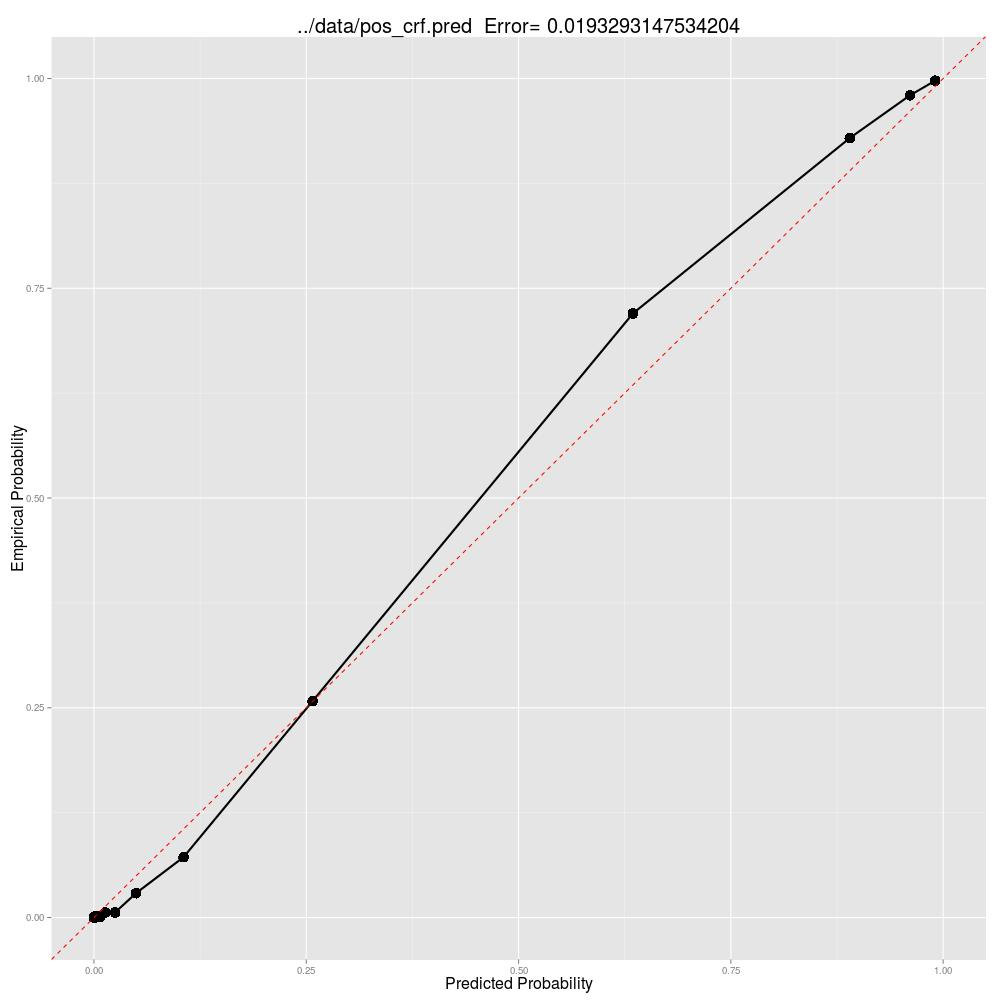
\includegraphics[width=\linewidth]{pos_crf_pred.jpg}
  \caption{Calibration curve for CRF-Basic (POS), Acc = ??, CalibScore = ??}
  \label{fig:pos_crf_pred}
\endminipage\hfill
\minipage{0.32\textwidth}
  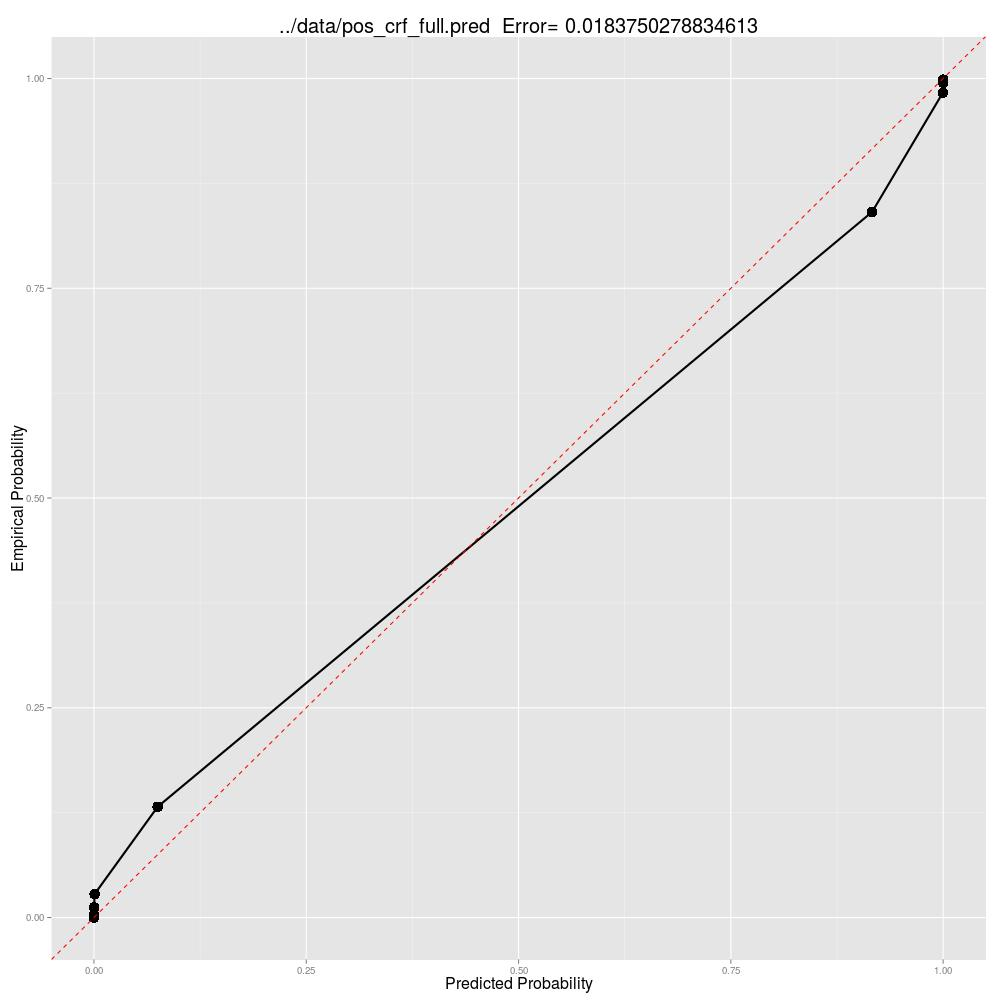
\includegraphics[width=\linewidth]{pos_crf_advanced_pred.jpg}
  \caption{Calibration curve for CRF-Advanced (POS), Acc = ??, CalibScore = ??}
  \label{fig:pos_crf_advanced_pred}  
\endminipage
\end{figure}

First of all, we compare a standard HMM with a CRF model with basic features (CRF-Basic). CRF-Basic contains only the emission features (pairs of the tag and the current token at each position) and the transition features (pairs of labels). Using CRF-Basic allows us to separate the characteristics of the model dependencies from the advantages of having features. The plots of calibration curves of the two models are shown in figure \ref{fig:pos_hmm_pred}. CRF-basic intuitively produces a better curve than HMM. Concretely, the miscalibration of CRF-Basic is roughly 1.8 times larger than that of HMM (0.019 vs. 0.035). Moreover, as seen from the distributions of points in the plots, CRF-Basic produces sharper predictions.

To measure fully the power of the CRF model, we add more features to it, including surrounding words, word shape, word length, prefixes and suffixes. This model, called CRF-Advanced, achieves a 96\% accuraccy on the task. It produces an extremely good posterior distribution. Figure \ref{fig:pos_crf_advanced_pred} shows its perfect calibration curve, which is just slightly off the perfect calibration line (calibration score = 0.018). 

\subsection{Twitter part-of-speech tagging}
\subsubsection{Data}

We repeat our comparision between HMMs and CRFs on a harder task, predicting POS tags for tweets. We use the ARK's Twitter POS data set (CITE NOAH), which consists of 1000 sentences for training, 327 sentences for development, 500 sentences for testing. The predictions we test is to predict whether a word has the ``V'' tag. 

\subsubsection{Data}

We conduct the same experiments as in Section BLAH BLAH and obtain similar patterns. CRF-Basic's miscalibration is about half HMM's (Figure \ref{fig:pos_tweet_hmm_pred}). On the other hand, equipped with better features, CRF-Advanced demonstrates a significant improvement from CRF-Basic, reducing further the miscalibration level by one half. It should also be noticed that CRF-Advanced does not give perfectly accurate predictions (87\% accuracy) but those are reliable predictions.   

\begin{figure}
\minipage{0.32\textwidth}
  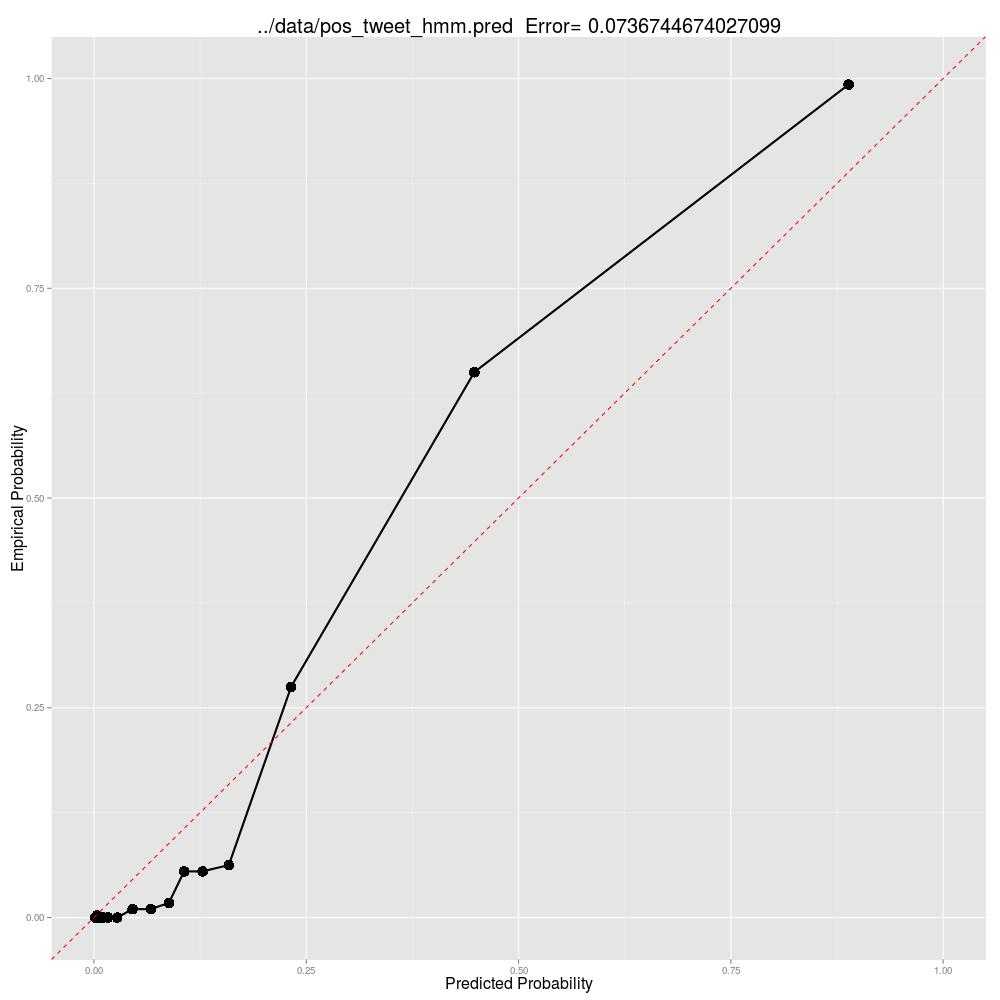
\includegraphics[width=\linewidth]{pos_tweet_hmm_pred.jpg}
  \caption{Calibration curve for HMM (POS Tweet), Acc = ??, CalibScore = ??}
  \label{fig:pos_tweet_hmm_pred}
\endminipage\hfill
\minipage{0.32\textwidth}
  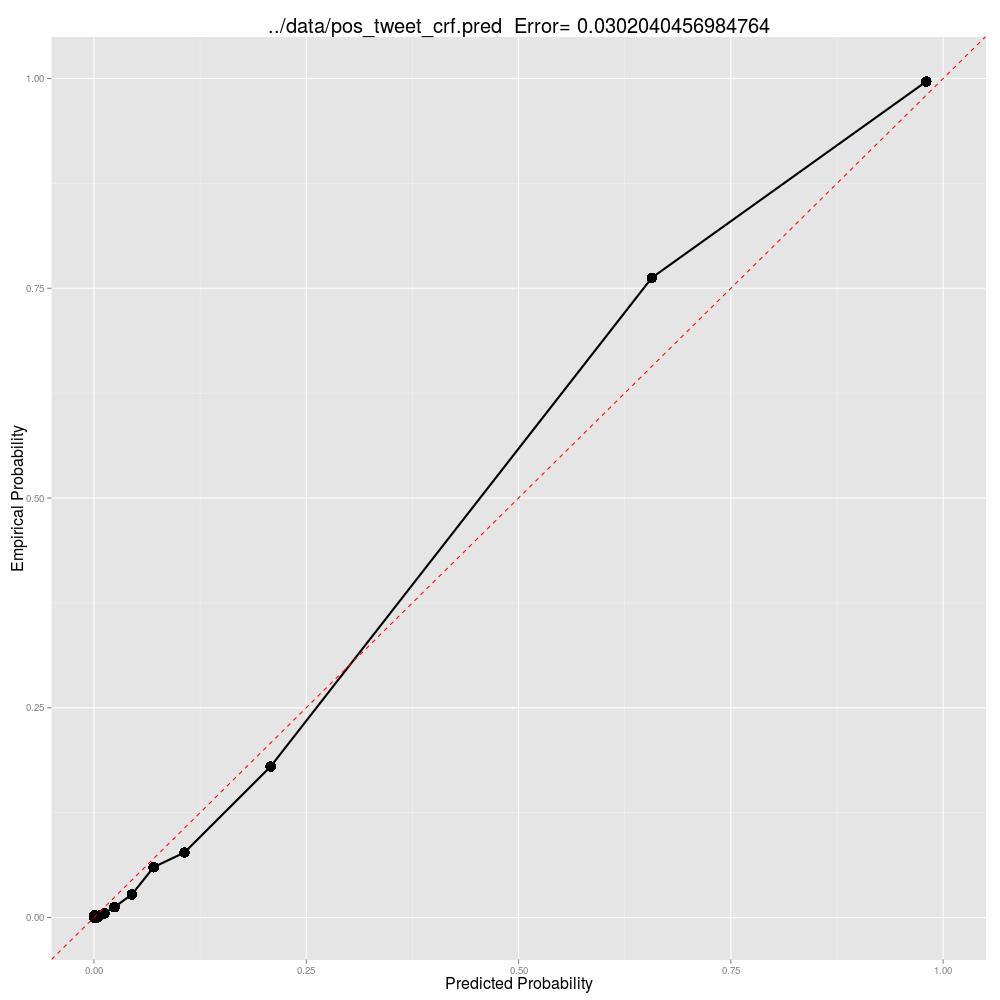
\includegraphics[width=\linewidth]{pos_tweet_crf_pred.jpg}
  \caption{Calibration curve for CRF-Basic (POS Tweet), Acc = ??, CalibScore = ??}
  \label{fig:pos_tweet_crf_pred} 
\endminipage\hfill
\minipage{0.32\textwidth}
  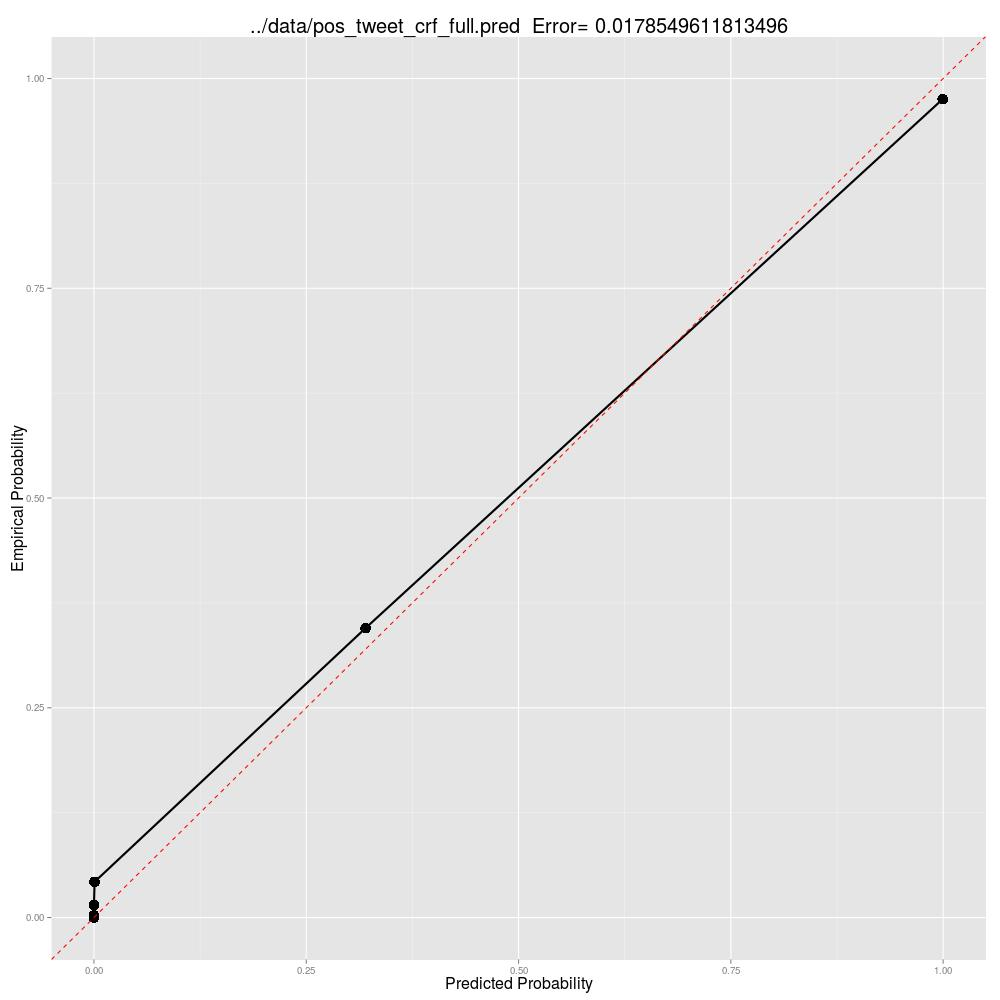
\includegraphics[width=\linewidth]{pos_tweet_crf_advanced_pred.jpg}
  \caption{Calibration curve for CRF-Advanced (POS Tweet), Acc = ??, CalibScore = ??}
  \label{fig:pos_tweet_advanced_crf_pred} 
\endminipage
\end{figure}

